%Your one page proposal should explicitly specify a title, the names of members of your group, the
%problem or question that your project addresses, the hypothesis that is being tested, the network 
%architecture and learning method(s) you will evaluate, the motivations for the evaluation, the 
%implementation language, the nature and source of the training data, and the evaluation design
%Your final report should include the same information, a tabulation of results, a discussion stating 
%your conclusions, and a short appendix with a sample run for each method you evaluate. Program 
%listings of software that you create are to be submitted separately

\documentclass{acm_proc_article-sp}
\usepackage[usenames,dvipsnames]{xcolor}
\usepackage{hyperref}
\usepackage{minted}
\usepackage{listings}
\usepackage{framed}

\newcommand{\todo}[1]{\textcolor{orange}{\textbf{TODO}: #1}} %~\\ 
\newcommand{\unsure}[1]{\textcolor{Mulberry}{\textbf{?} #1 \textbf{?}}}
\newcommand{\brainstorm}[1]{\textcolor{ProcessBlue}{\textbf{Brainstorming}: #1}}
\def\bs{\brainstorm}
\newcommand{\wordchoice}[1]{\textcolor{red}{\textbf{#1}}}
\def\wc{\wordchoice}

\definecolor{shadecolor}{rgb}{0.95,0.95,0.95}

\begin{document}

\title{Comparing Performances of Recurrent Jordan and Elman Neural Networks}
\numberofauthors{2}
\author{
\alignauthor James Parker\\%\titlenote{Dr.~Trovato insisted his name be first.}\\
       \affaddr{Department of Computer Science}\\
       \affaddr{University of Maryland, College Park}\\
       \affaddr{College Park, MD}\\
       \email{jp@jamesparker.me}
\alignauthor Kerry Cheng\\%\titlenote{Dr.~Trovato insisted his name be first.}\\
       \affaddr{Department of Computer Science}\\
       \affaddr{University of Maryland, College Park}\\
       \affaddr{College Park, MD}\\
       \email{kerry.cheng.2013@gmail.com}
}

\maketitle

\begin{abstract}
Jordan and Elman recurrent neural networks are two different methods to learn and predict about time series data. 
They both take similar approaches in that they both have context layers, but differ in how they update this layer. 
In this paper, we set out to compare the difference in performance between these two types of networks. %We fill this void by 
We accomplish this by implementing each network in the Julia language, and we test their errors on five different data sets. 


\todo{We find that: including results...}
\end{abstract}
\section{Introduction} % problem, solution, your contribution, outline
%\todo{mention supervised....}
Jordan and Elman networks are two forms of recurrent neural networks that share very similar behavior and functionality. 
They are both used to perform pattern recognition and time series forecasting given data over time. 
Jordan networks were first introduced by Jordan with the novel approach that the output of a neural network could be copied back to a new context layer in the network \cite{jordan}. Then the network could learn the associated weights of this new context layer by standard back propagation. 
Elman expanded on this idea by introducing Elman networks \cite{elman}. 
The difference with this new type of network is that the hidden layer is copied back to the context layer, instead of the output layer. 
Both of these networks seems to have a similar flavor in their approaches.
The problem is that there does not currently seem to be any detailed comparison on the performance of these two neural networks that covers many data sets. 

To fix this problem, we set out to perform a detailed comparison between Jordan and Elman recurrent neural networks. 
We began by implementing both network in the new programming language, Julia. 
We then train both types of networks on time varying input and output data while tuning training parameters to get best results. 
We chose five separate data sets to evaluate on, which all originate from the Matlab Neural Network Toolbox Sample Data Sets \cite{data}. 
These data sets were used to predict both continuous and discrete types of outputs.

This paper is laid out as follows. First we discuss our motivation for comparing Jordan and Elman networks in Julia. %for implementing Jordan and Elman networks in Julia
Then we cover the methods of our comparison, as well as the data sets used in our comparison. The next section goes over our results. Finally we discuss our results and draw conclusions.

\section{Motivation}
We decided to study Elman and Jordan networks because they are both standard techniques to perform training over time varying data. 
We are interested to see which network performs better, even though they take very similar approaches. 
Our hypothesis is that Elman networks should have higher performance than Jordan networks because intuitively, it seems like hidden layers contain more information than output layers. Since the context layers of Elman networks update from the hidden layer rather than the output layer, we expect the Elman networks to perform better. 

We also decided to implement these networks in Julia because it is a relatively new language that shows much potential for technical computing. 
For instance, it has features such as a rich type system and a JIT compiler \cite{julia}. 
Stronger types can help a programmer write more correct and less buggy code. 
The JIT compiler also offers huge speed improvements over interpretted languages like Matlab and R. 
For instance, quicksort in Julia is 105.09 times faster than Matlab's quicksort and is 517.34 times faster than R's quicksort. 
This is possible because instructions are compiled to machine operations instead of being evaluated within another language's interpretter.
Since the language is new, there are a limited number of packages available. Therefore our implementations may actually make an impact and be included as a standard Julia package. 

\begin{figure}
\begin{center}
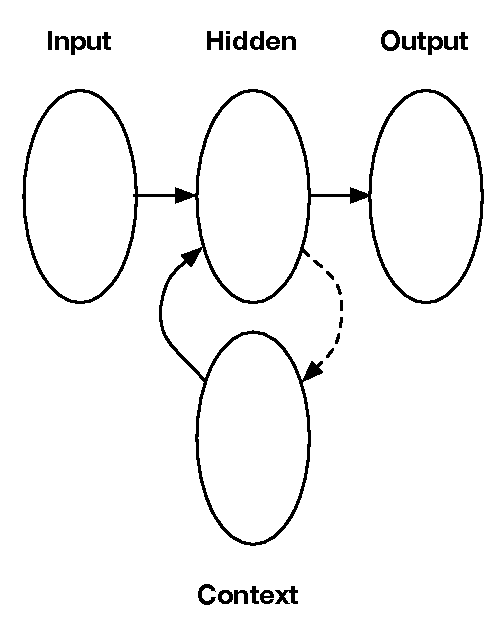
\includegraphics[scale=.8]{Images/elman.pdf}
\caption{The architecture of an Elman network.}
\label{fig:elman}
\end{center}
\end{figure}

\begin{figure}
\begin{center}
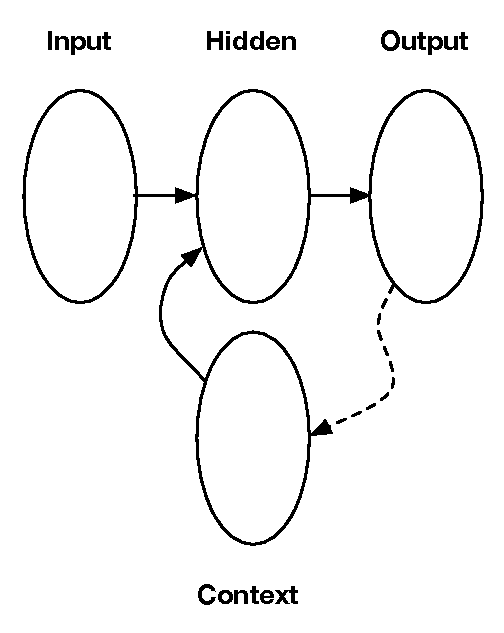
\includegraphics[scale=.8]{Images/jordan.pdf}
\caption{The architecture of a Jordan network.}
\label{fig:jordan}
\end{center}
\end{figure}

\section{Methods}
We implemented both Elman and Jordan recurrent neural networks in Julia. 
Each network's architecture can be seen in Figures \ref{fig:elman} and \ref{fig:jordan}, respectively. 
In the implementation, the networks are two layer in that they have one hidden layer. 
The size of the input and output layers are determined by the data set, while the user can define a desired number of hidden nodes. 
The size of the context layer is equal to either the size of the hidden layer or the output layer, depending on if the network is Elman or Jordan. 
In the figures, regular connections between layers are indicated by solid arrows, while backwards, copyback connections are dashed. 
The input layer also has a bias node whose activation is always one. 

The default activation rule is the logistic, or sigmoid function, however the user can specify an arbitrary activation rule to use by giving it (and its derivative) to the network. 
All of our comparison results used the logistic function for all layers of the network. 

For the learning rules, we used standard error back propagation to update the weight matrices. To update the context layer, we copyback by decaying the current context layer by a parameter $\mu$ and add either the hidden or output layer. For instance, the general learning rules for the implemented Elman networks are shown below, where $\eta$ is the learning rate, $f$ is the activation rule, and $C(t)$ is the context layer at a given time.
$$\Delta w_{ji} = \eta \delta_j a_i$$
$$\delta_{Oj} = f'(in_j)(c_{j}-a_{Oj})$$
$$\delta_{Hj} = f'(in_j) \sum_k w_{kj} \delta_k$$
$$C(t)_{j} = \mu * C(t-1)_j + a_{Hj}$$

The implementation also normalizes all of the input and output data to the interval $[0,1]$ during training. 
This is needed so that the network can learn about output data outside the iterval $[0,1]$. 
Normalizing the input also improves learning because then it is on a similar scale as the output. 

\begin{table}
\begin{center}
  \begin{tabular}{| c | c |}
  \hline
  \textbf{Liquid flow rate} & \textbf{Liquid temperature}\\ \hline
  0.3 & 98.628\\ \hline
  0.29297 & 98.646\\ \hline
  0.30356 & 98.638\\ \hline
  0.30653 & 98.621\\ \hline
  0.30216 & 98.614\\ \hline
  \end{tabular}
\end{center}  
  \caption{Heat exchanger data set.}
  \label{table:exchange}
\end{table}

To conduct our comparison of Elman and Jordan networks, we train each network on five different data sets. Each data set is split into training and test data, which allows us the record the network's perfomance in terms of the number of epochs, the training error, and the test error. Each epoch is one iteration through the sample training data. We measure error by taking the L2 norm.

All of the data sets used are time varying and come from the Matlab Neural Network Toolbox Sample Data Sets \cite{data}. 
There are three data sets that have continuous outputs. One is the heat exchanger data set, where the input is the liquid flow rate and the output is the liquid temperature. 
To give an idea of the data, the first few data points are shown in Table \ref{table:exchange}, where time moves down in the table. 
The next data set has outputs of the change in the world's total ice volume. % and no inputs. %Since there were no inputs, 
The input of the third data set is the electromagnetic current of a maglev train, while the output is the train's position.

We also analyzed two data sets with discrete, classification outputs. We could not find time varying, classification data sets so we created classifications out of the ones we were given. For instance, in the chicken pox data set, the number of cases of chicken pox per month in New York City is given. We then define an outbreak as true when the number of cases is above the average. This allowed us to treat the number of cases as the input, and whether there's an outbreak as the output. We use the same approach with the laser data set, which gives a laser's intensity over time. In this case, we classify a time step as either high or low intensity.

%\todo{network architecture - image, default use logistic/sigmoid activation, add a bias node to the input layer, discuss I/O data types?}
%\todo{nature and source of the training data - neural network }

\section{Results}

\begin{table}
\begin{center}
\begin{tabular}{cc|ccc|l}
\multicolumn{2}{ c }{Elman} & & \multicolumn{2}{ c }{Jordan} & \\ \cline{1-2} \cline{4-5}
\multicolumn{1}{ |c| }{$ \mu = .1 $} & 5000 & &
	\multicolumn{1}{ |c| }{$ \mu = .1 $} & 5000 & \\ \cline{2-2} \cline{5-5}
\multicolumn{1}{ |c| }{$ \eta = .1 $} & 0.02591 & &
	\multicolumn{1}{ |c| }{$ \eta = .1 $} & 0.04231 & \\ \cline{2-2} \cline{5-5}
\multicolumn{1}{ |c| }{$ |H| = 10 $} & 18.62037 & &
	\multicolumn{1}{ |c| }{$ |H| = 10 $} & 64.19846 & \\ \cline{1-2} \cline{4-5}

\multicolumn{1}{ |c| }{$ \mu = .3 $} & 5000 & &
	\multicolumn{1}{ |c| }{$ \mu = .3 $} & 5000 & \\ \cline{2-2} \cline{5-5}
\multicolumn{1}{ |c| }{$ \eta = .1 $} & 0.02270 & &
	\multicolumn{1}{ |c| }{$ \eta = .1 $} & 0.04551 & \\ \cline{2-2} \cline{5-5}
\multicolumn{1}{ |c| }{$ |H| = 10 $} & 21.73420 & &
	\multicolumn{1}{ |c| }{$ |H| = 10 $} & 80.20247 & \\ \cline{1-2} \cline{4-5}

\multicolumn{1}{ |c| }{$ \mu = .1 $} & 5000 & &
	\multicolumn{1}{ |c| }{$ \mu = .1 $} & 5000 & \\ \cline{2-2} \cline{5-5}
\multicolumn{1}{ |c| }{$ \eta = .3 $} & 0.02138 & &
	\multicolumn{1}{ |c| }{$ \eta = .3 $} & 0.04616 & \\ \cline{2-2} \cline{5-5}
\multicolumn{1}{ |c| }{$ |H| = 10 $} & 27.69586 & &
	\multicolumn{1}{ |c| }{$ |H| = 10 $} & 120.87661 & \\ \cline{1-2} \cline{4-5}

\multicolumn{1}{ |c| }{$ \mu = .1 $} & 5000 & &
	\multicolumn{1}{ |c| }{$ \mu = .1 $} & 5000 & \\ \cline{2-2} \cline{5-5}
\multicolumn{1}{ |c| }{$ \eta = .3 $} & 0.01939 & &
	\multicolumn{1}{ |c| }{$ \eta = .3 $} & 0.04270 & \\ \cline{2-2} \cline{5-5}
\multicolumn{1}{ |c| }{$ |H| = 20 $} & 24.62165 & &
	\multicolumn{1}{ |c| }{$ |H| = 20 $} & 135.60854 & \\ \cline{1-2} \cline{4-5}
\end{tabular}
\end{center}  
  \caption{The number of epochs, the training error, and test error for the heat exchanger data set.}
  \label{table:exchangeresults}
\end{table}


\begin{table}
\begin{center}
\begin{tabular}{cc|ccc|l}
\multicolumn{2}{ c }{Elman} & & \multicolumn{2}{ c }{Jordan} & \\ \cline{1-2} \cline{4-5}
\multicolumn{1}{ |c| }{$ \mu = .3 $} & 5000 & &
	\multicolumn{1}{ |c| }{$ \mu = .3 $} & 5000 & \\ \cline{2-2} \cline{5-5}
\multicolumn{1}{ |c| }{$ \eta = .5 $} & 0.10252 & &
	\multicolumn{1}{ |c| }{$ \eta = .5 $} & 0.13473 & \\ \cline{2-2} \cline{5-5}
\multicolumn{1}{ |c| }{$ |H| = 10 $} & 12.45976 & &
	\multicolumn{1}{ |c| }{$ |H| = 10 $} & 13.65836 & \\ \cline{1-2} \cline{4-5}

\multicolumn{1}{ |c| }{$ \mu = .1 $} & 5000 & &
	\multicolumn{1}{ |c| }{$ \mu = .1 $} & 5000 & \\ \cline{2-2} \cline{5-5}
\multicolumn{1}{ |c| }{$ \eta = .5 $} & 0.09848 & &
	\multicolumn{1}{ |c| }{$ \eta = .5 $} & 0.14861 & \\ \cline{2-2} \cline{5-5}
\multicolumn{1}{ |c| }{$ |H| = 10 $} & 12.75804 & &
	\multicolumn{1}{ |c| }{$ |H| = 10 $} & 11.44808 & \\ \cline{1-2} \cline{4-5}

\multicolumn{1}{ |c| }{$ \mu = .1 $} & 5000 & &
	\multicolumn{1}{ |c| }{$ \mu = .1 $} & 5000 & \\ \cline{2-2} \cline{5-5}
\multicolumn{1}{ |c| }{$ \eta = .3 $} & 0.12102 & &
	\multicolumn{1}{ |c| }{$ \eta = .3 $} & 0.16781 & \\ \cline{2-2} \cline{5-5}
\multicolumn{1}{ |c| }{$ |H| = 10 $} & 11.92459 & &
	\multicolumn{1}{ |c| }{$ |H| = 10 $} & 11.26288 & \\ \cline{1-2} \cline{4-5}

\multicolumn{1}{ |c| }{$ \mu = .1 $} & 5000 & &
	\multicolumn{1}{ |c| }{$ \mu = .1 $} & 5000 & \\ \cline{2-2} \cline{5-5}
\multicolumn{1}{ |c| }{$ \eta = .3 $} & 0.09366 & &
	\multicolumn{1}{ |c| }{$ \eta = .3 $} & 0.12934 & \\ \cline{2-2} \cline{5-5}
\multicolumn{1}{ |c| }{$ |H| = 20 $} & 13.13796 & &
	\multicolumn{1}{ |c| }{$ |H| = 20 $} & 14.52611 & \\ \cline{1-2} \cline{4-5}
\end{tabular}
\end{center}  
  \caption{The number of epochs, the training error, and test error for the ice data set.}
  \label{table:iceresults}
\end{table}


\begin{table}
\begin{center}
\begin{tabular}{cc|ccc|l}
\multicolumn{2}{ c }{Elman} & & \multicolumn{2}{ c }{Jordan} & \\ \cline{1-2} \cline{4-5}
\multicolumn{1}{ |c| }{$ \mu = .1 $} & 5000 & &
	\multicolumn{1}{ |c| }{$ \mu = .1 $} & 5000 & \\ \cline{2-2} \cline{5-5}
\multicolumn{1}{ |c| }{$ \eta = .3 $} & 0.01731 & &
	\multicolumn{1}{ |c| }{$ \eta = .3 $} & 0.02495 & \\ \cline{2-2} \cline{5-5}
\multicolumn{1}{ |c| }{$ |H| = 10 $} & 61.55067 & &
	\multicolumn{1}{ |c| }{$ |H| = 10 $} & 67.65677 & \\ \cline{1-2} \cline{4-5}

\multicolumn{1}{ |c| }{$ \mu = .1 $} & 146 & &
	\multicolumn{1}{ |c| }{$ \mu = .1 $} & 5000 & \\ \cline{2-2} \cline{5-5}
\multicolumn{1}{ |c| }{$ \eta = .3 $} & 0.00999 & &
	\multicolumn{1}{ |c| }{$ \eta = .3 $} & 0.01638 & \\ \cline{2-2} \cline{5-5}
\multicolumn{1}{ |c| }{$ |H| = 20 $} & 65.29465 & &
	\multicolumn{1}{ |c| }{$ |H| = 20 $} & 65.38774 & \\ \cline{1-2} \cline{4-5}

\multicolumn{1}{ |c| }{$ \mu = .1 $} & 80 & &
	\multicolumn{1}{ |c| }{$ \mu = .1 $} & 5000 & \\ \cline{2-2} \cline{5-5}
\multicolumn{1}{ |c| }{$ \eta = .3 $} & 0.00994 & &
	\multicolumn{1}{ |c| }{$ \eta = .3 $} & 0.01045 & \\ \cline{2-2} \cline{5-5}
\multicolumn{1}{ |c| }{$ |H| = 30 $} & 68.57120 & &
	\multicolumn{1}{ |c| }{$ |H| = 30 $} & 64.22677 & \\ \cline{1-2} \cline{4-5}

\multicolumn{1}{ |c| }{$ \mu = .1 $} & 5000 & &
	\multicolumn{1}{ |c| }{$ \mu = .1 $} & 5000 & \\ \cline{2-2} \cline{5-5}
\multicolumn{1}{ |c| }{$ \eta = .3 $} & 0.00509 & &
	\multicolumn{1}{ |c| }{$ \eta = .3 $} & 0.01045 & * \\ \cline{2-2} \cline{5-5}
\multicolumn{1}{ |c| }{$ |H| = 30 $} & 60.43116 & &
	\multicolumn{1}{ |c| }{$ |H| = 30 $} & 64.22677 & \\ \cline{1-2} \cline{4-5}
\end{tabular}
\end{center}  
  \caption{The number of epochs, the training error, and test error for the maglev data set.}
  \label{table:maglevresults}
\end{table}


\begin{table}
\begin{center}
\begin{tabular}{cc|ccc|l}
\multicolumn{2}{ c }{Elman} & & \multicolumn{2}{ c }{Jordan} & \\ \cline{1-2} \cline{4-5}
\multicolumn{1}{ |c| }{$ \mu = .1 $} & 5000 & &
	\multicolumn{1}{ |c| }{$ \mu = .1 $} & 5000 & \\ \cline{2-2} \cline{5-5}
\multicolumn{1}{ |c| }{$ \eta = .3 $} & 0.04758 & &
	\multicolumn{1}{ |c| }{$ \eta = .3 $} & 0.05300 & \\ \cline{2-2} \cline{5-5}
\multicolumn{1}{ |c| }{$ |H| = 10 $} & 3.76940 & &
	\multicolumn{1}{ |c| }{$ |H| = 10 $} & 2.47227 & \\ \cline{1-2} \cline{4-5}

\multicolumn{1}{ |c| }{$ \mu = .1 $} & 5000 & &
	\multicolumn{1}{ |c| }{$ \mu = .1 $} & 5000 & \\ \cline{2-2} \cline{5-5}
\multicolumn{1}{ |c| }{$ \eta = .3 $} & 0.03121 & &
	\multicolumn{1}{ |c| }{$ \eta = .3 $} & 0.08092 & \\ \cline{2-2} \cline{5-5}
\multicolumn{1}{ |c| }{$ |H| = 20 $} & 3.30458 & &
	\multicolumn{1}{ |c| }{$ |H| = 20 $} & 2.19778 & \\ \cline{1-2} \cline{4-5}

\multicolumn{1}{ |c| }{$ \mu = 0 $} & 5000 & &
	\multicolumn{1}{ |c| }{$ \mu = 0 $} & 5000 & \\ \cline{2-2} \cline{5-5}
\multicolumn{1}{ |c| }{$ \eta = .3 $} & 0.03466 & &
	\multicolumn{1}{ |c| }{$ \eta = .3 $} & 0.08059 & \\ \cline{2-2} \cline{5-5}
\multicolumn{1}{ |c| }{$ |H| = 20 $} & 3.37411 & &
	\multicolumn{1}{ |c| }{$ |H| = 20 $} & 2.21680 & \\ \cline{1-2} \cline{4-5}
\end{tabular}
\end{center}  
  \caption{The number of epochs, the training error, and test error for the chickenpox data set.}
  \label{table:poxresults}
\end{table}


\begin{table}
\begin{center}
\begin{tabular}{cc|ccc|l}
\multicolumn{2}{ c }{Elman} & & \multicolumn{2}{ c }{Jordan} & \\ \cline{1-2} \cline{4-5}
\multicolumn{1}{ |c| }{$ \mu = .1 $} & 5000 & &
	\multicolumn{1}{ |c| }{$ \mu = .1 $} & 5000 & \\ \cline{2-2} \cline{5-5}
\multicolumn{1}{ |c| }{$ \eta = .3 $} & 0.08570 & &
	\multicolumn{1}{ |c| }{$ \eta = .3 $} & 0.08453 & \\ \cline{2-2} \cline{5-5}
\multicolumn{1}{ |c| }{$ |H| = 10 $} & 8.51078 & &
	\multicolumn{1}{ |c| }{$ |H| = 10 $} & 7.26211 & \\ \cline{1-2} \cline{4-5}

\multicolumn{1}{ |c| }{$ \mu = 0 $} & 5000 & &
	\multicolumn{1}{ |c| }{$ \mu = 0 $} & 5000 & \\ \cline{2-2} \cline{5-5}
\multicolumn{1}{ |c| }{$ \eta = .3 $} & 0.08566 & &
	\multicolumn{1}{ |c| }{$ \eta = .3 $} & 0.08439 & \\ \cline{2-2} \cline{5-5}
\multicolumn{1}{ |c| }{$ |H| = 10 $} & 8.76133 & &
	\multicolumn{1}{ |c| }{$ |H| = 10 $} & 7.25134 & \\ \cline{1-2} \cline{4-5}
\end{tabular}
\end{center}  
  \caption{The number of epochs, the training error, and test error for the laser intensity data set.}
  \label{table:laserresults}
\end{table}

\section{Discussion}

... There are a few other that have looked at these two networks???


\bibliographystyle{plain}
\bibliography{myrefs.bib}

\appendix

\section{Sample runs}

\begin{listing}
\begin{snugshade}
\begin{verbatim}
require("../src/RNN.jl")
require("../src/ElmanRNN.jl")
require("helper.jl")
using RNN
using ElmanRNN

srand(63)

data = importData("exchanger")
dataInput = data[:,1]
dataOutput = data[:,2]

trainingIndices = 1:2000
testIndices = 2001:4000

trainingInput = TimeSeriesSample( 
    dataInput[trainingIndices])
trainingInputs = TimeSeriesSamples( 
    [trainingInput])
trainingOutput = TimeSeriesSample( 
    dataOutput[trainingIndices])
trainingOutputs = TimeSeriesSamples( 
    [trainingOutput])

testInput = TimeSeriesSample( 
    dataInput[testIndices])
testInputs = TimeSeriesSamples( [testInput])
testOutput = TimeSeriesSample( 
    dataOutput[testIndices])
testOutputs = TimeSeriesSamples( [testOutput])

net = ElmanNetwork(1, 20, 1)
net.mu = .1
net.eta = .3
net.errorThreshold = .01
numEpochs, lastTrainingError = ElmanTrain!(
    net, trainingInputs, trainingOutputs)

target = ElmanEvaluate( net, testInput)
testError = norm(target - testOutput.sample)

print("Num Epochs: $numEpochs\n")
print("Last Training Error: $lastTrainingError\n")
print("Testing Error: $testError\n")
\end{verbatim}
\end{snugshade}
\caption{Sample Elman run with heat exchanger data set.}
\label{code:exchangerElman}
\end{listing}

\begin{listing}
\begin{snugshade}
\begin{verbatim}
require("../src/RNN.jl")
require("../src/JordanRNN.jl")
require("helper.jl")
using RNN
using JordanRNN

srand(63)

data = importData("exchanger")
dataInput = data[:,1]
dataOutput = data[:,2]

trainingIndices = 1:2000
testIndices = 2001:4000

trainingInput = TimeSeriesSample( 
    dataInput[trainingIndices])
trainingInputs = TimeSeriesSamples( [trainingInput])
trainingOutput = TimeSeriesSample( 
    dataOutput[trainingIndices])
trainingOutputs = TimeSeriesSamples( 
    [trainingOutput])

testInput = TimeSeriesSample( 
    dataInput[testIndices])
testInputs = TimeSeriesSamples( [testInput])
testOutput = TimeSeriesSample( 
    dataOutput[testIndices])
testOutputs = TimeSeriesSamples( [testOutput])

net = JordanNetwork(1, 20, 1)
net.mu = .1
net.eta = .3
net.errorThreshold = .01
numEpochs, lastTrainingError = JordanTrain!( net, 
    trainingInputs, trainingOutputs)

target = JordanEvaluate( net, testInput)
testError = norm(target - testOutput.sample)

print("Num Epochs: $numEpochs\n")
print("Last Training Error: $lastTrainingError\n")
print("Testing Error: $testError\n")
\end{verbatim}
\end{snugshade}
\caption{Sample Jordan run with heat exchanger data set.}
\label{code:exchangerJordan}
\end{listing}

\end{document}